%%%%%%%%%%%%%%%%%%%%%%%%%%%%%%%%%%%%%%%%%%%%%%%%%%%%%%%%%%%%%%%%%%%%%
%
% Complete documentation on the extended LaTeX markup used for Insight
% documentation is available in ``Documenting Insight'', that is part
% of the standard documentation for Insight.  It may be found online
% at:
%
%                    http://www.itk.org
%
%%%%%%%%%%%%%%%%%%%%%%%%%%%%%%%%%%%%%%%%%%%%%%%%%%%%%%%%%%%%%%%%%%%%%

\documentclass{InsightSoftwareGuide}


\usepackage[dvips]{graphicx}
\usepackage{times,lscape,url}
%\usepackage{mdwtab}


%%% \usepackage[latin1]{inputenc}
%%% \selectlanguage{french}
% Configuration pour les accents francais pour l'OTB
\usepackage[latin1]{inputenc}
%\usepackage[french]{babel}
\usepackage{tikz}


\usepackage{color}

\definecolor{listcomment}{rgb}{0.0,0.5,0.0}
\definecolor{listkeyword}{rgb}{0.0,0.0,0.5}
\definecolor{listnumbers}{gray}{0.65}
\definecolor{listlightgray}{gray}{0.955}
\definecolor{listwhite}{gray}{1.0}

\usepackage{listings}
\newcommand{\lstsetcpp}
{
\lstset{frame = tb,
       framerule = 0.25pt,
       float,
       fontadjust,
       backgroundcolor={\color{listlightgray}},
       basicstyle = {\ttfamily\footnotesize},
       keywordstyle = {\ttfamily\color{listkeyword}\textbf},
       identifierstyle = {\ttfamily},
       commentstyle = {\ttfamily\color{listcomment}\textit},
       stringstyle = {\ttfamily},
       showstringspaces = false,
       showtabs = false,
       numbers = none,
       numbersep = 6pt,
       numberstyle={\ttfamily\color{listnumbers}},
       tabsize = 2,
       language=[ANSI]C++,
       floatplacement=!h
       }
}
\newcommand{\lstsetpython}
{
\lstset{language=Python
        }
}
\newcommand{\lstsetjava}
{
\lstset{language=Java
        }
}


\newif\ifitkFullVersion
\itkFullVersiontrue
%\itkFullVersionfalse

\newif\ifitkPrintedVersion
\itkPrintedVersiontrue
%\itkPrintedVersionfalse


%%%%%%%%%%%%%%%%%%%%%%%%%%%%%%%%%%%%%%%%%%%%%%%%%%%%%%%%%%%%%%%%%%
%
%  hyperref should be the last package to be loaded.
%
%%%%%%%%%%%%%%%%%%%%%%%%%%%%%%%%%%%%%%%%%%%%%%%%%%%%%%%%%%%%%%%%%%
\ifitkPrintedVersion
\usepackage[dvips,
pdftitle={Monteverdi Guide},
pdfauthor={CNES},
pdfsubject={Remote Sensing, Orfeo, Pleiades, Cosmo Skymed},
pdfkeywords={image processing, Remote sensing, Guide},
pdfpagemode={UseOutlines},
bookmarks,bookmarksopen,
pdfstartview={FitH},
backref,
colorlinks,linkcolor={black},citecolor={black},urlcolor={black},
]{hyperref}
\else
\usepackage[dvips,
pdftitle={Monteverdi Guide},
pdfauthor={CNES},
pdfsubject={Remote Sensing, Orfeo, Pleiades, Cosmo Skymed},
pdfkeywords={image processing, Remote sensing, Guide},
pdfpagemode={UseOutlines},
bookmarks,bookmarksopen,
pdfstartview={FitH},
backref,
colorlinks,linkcolor={blue},citecolor={blue},urlcolor={blue},
]{hyperref}
\fi

\usepackage{amsmath,amssymb,amsfonts}
\usepackage{bbm}
%%%%%%%%%%%%%%%%%%%%%%%%%%%%%%%%%%%%%%%%%%%%%%%%%%%%%%%%%%%%%%%%%%%
%
%
%   Load configuration parameters prepared by CMake
%
%
%%%%%%%%%%%%%%%%%%%%%%%%%%%%%%%%%%%%%%%%%%%%%%%%%%%%%%%%%%%%%%%%%%%

% Define where in the disk is the Insight source tree 
\def\ITKSOURCEDIR{}
\graphicspath{{/home/ORFEO/thomas/ORFEO-TOOLBOX/OTB-Documents/SoftwareGuide/Art/}{/home/ORFEO/thomas/ORFEO-TOOLBOX/OTB-Documents/SoftwareGuide/Art/}}
\def\bibtexdatabasepath{/home/ORFEO/thomas/ORFEO-TOOLBOX/OTB-Documents/SoftwareGuide/../Latex/Insight}


% Define command to make reference to on-line Doxygen documentation
\newcommand{\doxygen}[1]{
\href{http://www.itk.org/Doxygen/html/classitk_1_1#1.html}{\code{itk::#1}}}  

% Define command to make reference to on-line Doxygen documentation
\newcommand{\subdoxygen}[2]{
\href{http://www.itk.org/Doxygen/html/classitk_1_1#1_1_1#2.html}{\code{itk::#1::#2}}}  

% Define command for the standard comment introducing classes with similar functionalities
\newcommand{\relatedClasses}{
\textbf{The following classes provide similar functionality:}}


\def\logoCNES{CNES_nom.eps}

\newtheorem{algo}{Algorithm}
\newtheorem{defin}{Definition}
%%%%%%%%%%%%%%%%%%%%%%%%%%%%%%%%%%%%%%%%%%%%%%%%%%%%%%%%%%%%%%%%%%%
%
%
%           The Insight Toolkit Software Guide
%
%
%%%%%%%%%%%%%%%%%%%%%%%%%%%%%%%%%%%%%%%%%%%%%%%%%%%%%%%%%%%%%%%%%%%

\title{The Monteverdi Guide\\ Updated
  for OTB-3.2}

\author{OTB Development Team}

\authoraddress{
  \url{http://www.orfeo-toolbox.org}\\
  e-mail: \email{otb@cnes.fr}
}

\date{\today}


% actually write the .idx file
\makeindex

\setcounter{tocdepth}{3}



%%%%%%%%%%%%%%%%%%%%%%%%%%%%%%%%%%%%%%%%%%%%%%%%%%%%%%%%%%%%%%%%%%%
%
%           Begin Document
%
%%%%%%%%%%%%%%%%%%%%%%%%%%%%%%%%%%%%%%%%%%%%%%%%%%%%%%%%%%%%%%%%%%%

\begin{document}

\ifitkPrintedVersion
%% 
\begin{minipage}[t][3cm][b]{\textwidth}
\rule{14cm}{1pt}
\end{minipage}


\begin{minipage}[t][3cm][b]{\textwidth}
\Huge
The ITK Software Guide\\
\normalsize
\par
\emph{updated for version 2.4}\\
\end{minipage}

\hfill
\begin{minipage}[t][6cm][b]{0.6\textwidth}
\Large
\renewcommand{\baselinestretch}{1.5}
Luis Ib\'{a}\~{n}ez\\
Will Schroeder\\
Lydia Ng\\
Josh Cates\\
and the \emph{Insight Software Consortium}
\normalsize
\end{minipage}


\begin{minipage}[t][2cm][b]{\textwidth}
\rule{14cm}{1pt}
\end{minipage}

\newpage

\begin{minipage}[t][4cm][b]{\textwidth}
\begin{center}

\includegraphics[width=0.5\textwidth]{Kitware-logo-medium-res.eps}
\end{center}
\par
\begin{center}
\large
\copyright 2003 Kitware, Inc. \emph{(cover, preface, postface)}\\
\copyright 2003 Insight Software Consortium \emph{(main text body)}\\
Published by Kitware, Inc. \texttt{http://www.kitware.com}
\normalsize
\end{center}
\end{minipage}


\begin{minipage}[t][2.25cm][b]{\textwidth}
\begin{center}
All rights reserved. No part of this book may be reproduced, in any form 
or by any means, without the express written permission of the copyright
holders. An electronic version of this document is available from
\texttt{http://www.itk.org} and may be used under the provisions of the
ITK copyright found at \texttt{http://www.itk.org/HTML/Copyright.htm}.
\end{center}
\end{minipage}


\begin{minipage}[t][3.2cm][b]{\textwidth}
\begin{center}
The publisher Kitware, Inc. offers discounts on this book when ordered in
bulk quantities.\\
The publisher also produces companion works to this text such as \emph{The
Visualization Toolkit An Object-Oriented Approach to 3D Graphics 3rd Edition}
by Schroeder, Martin and Lorensen, \emph{Mastering CMake} by Martin and
Hoffman and \emph{The VTK's Users Guide} by Kitware.\\
For more information contact Kitware, Inc at \texttt{kitware@kitware.com}.\\
You may also order directly from Kitware's electronic store at
\texttt{http://www.kitware.com/products}\\
\end{center}
\end{minipage}

\begin{minipage}[t][2.7cm][b]{\textwidth}
\begin{center}
Contributors to this work include those listed on the title page as well
as:\\ Cover Design: Luis Ib\'{a}\~{n}ez and S\'{e}bastien Barr\'{e}\\
Technical Contributors: World-Wide ITK Developer Community at
\texttt{www.itk.org}. \\Document created with \LaTeX{}, using CMake as
configuration manager, with a Perl script to extract examples from the
\code{Insight/Examples} directory. All code in this document compiled at
the time of publication.
\end{center}
\end{minipage}


\begin{minipage}[t][2.5cm][b]{\textwidth}
\begin{center}
This project has been funded in whole or in part with Federal funds from the
National Institutes of Health (NLM, NIDCR, NIMH, NEI, NINDS, NIDCD, NCI), the
NSF, and the DoD (TATRC) under the direction of the National Library of
Medicine, National Institutes of Health, contracts number N01-LM-9-3531,
N01-LM-9-3532, N01-LM-0-3501, N01-LM-0-3502, N01-LM-0-3503, and
N01-LM-0-3504.
\end{center}
\end{minipage}


\begin{minipage}[t][1.0cm][b]{\textwidth}
\begin{center}
All product names mentioned herein are the trademarks of their respective 
owners.
\end{center}
\end{minipage}


\begin{minipage}[t][1.0cm][b]{\textwidth}
\begin{center}
Printed and produced in the United States of America.\\
ISBN 1-930934-15-7
\end{center}
\end{minipage}

\fi

\maketitle

\frontmatter

\hyperbaseurl{http://www.orfeo-toolbox.org}

\lstsetcpp


%%%%%%%%%%%%%%%%%%%%%%%%%%%%%%%%%%%%%%%%%%
%
%  Page with OTB logo
%
%%%%%%%%%%%%%%%%%%%%%%%%%%%%%%%%%%%%%%%%%%
\cleardoublepage

\begin{minipage}[t][10cm][b]{\textwidth}
\center

\includegraphics[width=0.5\textwidth]{logoVectoriel.eps}
\large
\begin{center}
\emph{The ORFEO Toolbox is not a black box.}\\
\end{center}
\hspace{8cm} Ch.D.
\normalsize
\end{minipage}



%%%%%%%%%%%%%%%%%%%%%%%%%%%%%%%%%%%%%%%%%%%%%%
%
% remove headings from the following material
\pagestyle{plain}
%
%%%%%%%%%%%%%%%%%%%%%%%%%%%%%%%%%%%%%%%%%%%%%%



%%\ifitkPrintedVersion
%% % We want this material to fit on two pages
\small

\chapter*{About the Cover}

Creating the cover image demonstrating the capabilities of the toolkit was a
challenging task.\footnote{The source code for the cover is available from
InsightDocuments/SoftwareGuide/Cover/Source/.} Given that the origins of ITK
are with the Visible Human Project it seemed appropriate to create an image
utilizing the VHP data sets, and it was decided to use the more recently
acquired Visible Woman dataset.  Both the RGB cryosections and the CT scans
were combined in the same scene.

\begin{description}

\item [Removing the Gel.]
The body of the Visible Woman was immersed in a block of gel during the
freezing process. This gel appears as a blue material in the cryogenic data.
To remove the gel, the joint histogram of RGB values was computed. This
resulted in an 3D image of $256\times256\times256$ pixels. The histogram
image was visualized in VolView.\footnote{VolView is a commercial product
from Kitware. It supports ITK plug-ins and is available as a free viewer or
may be licensed with advanced functionality. See
http://www.kitware.com/products/volview.html for information.} The cluster
corresponding to the statistical distribution of blue values was identified
visually, and a separating plane was manually defined in RGB space. The
equation of this plane was subsequently used to discriminate pixels in the
gel from pixels in the anatomical structures. The gel pixels were zeroed out
and the RGB values on the body were preserved.

\item[The Skin.]
The skin was easy to segment once the gel was removed. A simple region
growing algorithm was used requiring seed points in the region previously
occupied by the gel and then set to zero values. An anti-aliasing filter was
applied in order to generate an image of pixel type float where the surface
was represented by the zero set. This data set was exported to VTK where a
contouring filter was used to extract the surface and introduce it in the VTK
visualization pipeline.

\item[The Brain.]
The visible part of the brain represents the surface of the gray matter.  The
brain was segmented using the vector version of the confidence connected
image filter.  This filter implements a region growing algorithm that starts
from a set of seed points and adds neighboring pixels subject to a condition
of homogeneity.

The set of sparse points obtained from the region growing algorithm was
passed through a mathematical morphology dilation in order to close holes and
then through a binary median filter. The binary median filter has the
outstanding characteristic of being very simple in implementation by applying
a sophisticated effect on the image. Qualitatively it is equivalent to a
curvature flow evolution of the iso-contours. In fact the binary median
filter as implemented in ITK is equivalent to the majority filter that
belongs to the family of voting filters classified as a subset of the
\emph{Larger than Life} cellular automata. Finally, the volume resulting from
the median filter was passed through the anti-aliasing image filter. As
before, VTK was used to extract the surface.

\item[The Neck Musculature.]
The neck musculature was not perfectly segmented. Indeed, the resulting
surface is a fusion of muscles, blood vessels and other anatomical
structures. The segmentation was performed by applying the
VectorConfidenceConnectedImageFilter to the cryogenic dataset. Approximately
60 seed points were manually selected and then passed to the filter as
input. The binary mask produced by the filter was dilated with a mathematical
morphology filter and smoothed with the BinaryMedianImageFilter. The
AntiAliasBinaryImageFilter was used at the end to reduce the pixelization
effects prior to the extraction of the iso-surface with vtkContourFilter.

\item[The Skull.]
The skull was segmented from the CT data set and registered to the cryogenic
data. The segmentation was performed by simple thresholding, which was good
enough for the cover image. As a result, most of the bone structures are
actually fused together. This includes the jaw bone and the cervical
vertebrae.

\item[The Eye.] 
The eye is charged with symbolism in this image. This is due in part because
the motivation for the toolkit is the analysis of the Visible Human data,
and in part because the name of the toolkit is \emph{Insight}.

The first step in processing the eye was to extract a sub-image of
$60\times60\times60$ pixels centered around the eyeball from the RGB
cryogenic data set. This small volume was then processed with the vector
gradient anisotropic diffusion filter in order to increase the homogeneity of
the pixels in the eyeball.

The smoothed volume was segmented using the
VectorConfidenceConnectedImageFilter using 10 seed points. The resulting
binary mask was dilated with a mathematical morphology filter with a
structuring element of radius one, then smoothed with a binary mean image
filter (equivalent to majority voting cellular automata). Finally the mask
was processed with the AntiAliasBinaryImageFilter in order to generate a
float image with the eyeball contour embedded as a zero set.

\item[Visualization.]
The visualization of the segmentation was done by passing all the binary
masks through the AntiAliasBinaryImageFilter, generating iso-contours with
VTK filters, and then setting up a VTK Tcl script. The skin surface was
clipped using the vtkClipPolyDataFilter using the implicit function
vtkCylinder. The vtkWindowToImageFilter proved to be quite useful for
generating the final high resolution rendering of the scene ($3000\times3000$
pixels).

\item[Cosmetic Postprocessing.]
We have to confess that we used Adobe Photoshop to post-process the image. In
particular, the background of the image was adjusted using Photoshop's color
selection. The overall composition of the image with the cover text and
graphics was also performed using Photoshop.

\end{description}

\normalsize

%%\fi

%\chapter*{Foreword}
\noindent


Beside the Pleiades (PHR) and Cosmo-Skymed (CSK) systems developments
forming ORFEO, the dual and bilateral system (France - Italy) for
Earth Observation, the ORFEO Accompaniment Program was set up, to
prepare, accompany and promote the use and the exploitation of the
images derived from these sensors.

The creation of a preparatory
program\footnote{http://smsc.cnes.fr/PLEIADES/A\_prog\_accomp.htm} is
needed because of:
\begin{itemize}
\item the new capabilities and performances of the ORFEO systems
  (optical and radar high resolution, access capability, data quality,
  possibility to acquire simultaneously in optic and radar),
\item the implied need of new methodological developments : new
  processing methods, or adaptation of existing methods,
\item the need to realise those new developments in very close
  cooperation with the final users for better integration of new
  products in their systems.

\end{itemize}

This program was initiated by CNES mid-2003 and will last until mid
2013.  It consists in two parts, between which it is necessary to keep
a strong interaction:
\begin{itemize}
\item A Thematic part,
\item A Methodological part.
\end{itemize}

The Thematic part covers a large range of applications (civil and
defence), and aims at specifying and validating value added products
and services required by end users. This part includes consideration
about products integration in the operational systems or processing
chains. It also includes a careful thought on intermediary structures
to be developed to help non-autonomous users. Lastly, this part aims
at raising future users awareness, through practical demonstrations
and validations.

The Methodological part objective is the definition and the
development of tools for the operational exploitation of the
submetric optic and radar images (tridimensional aspects, changes
detection, texture analysis, pattern matching, optic radar
complementarities). It is mainly based on R\&D studies and doctorate
and post-doctorate researches.

In this context, CNES\footnote{http://www.cnes.fr} decided to develop
the \emph{ORFEO ToolBox} (OTB), a set of algorithms encapsulated in a
software library. The goals of the OTB is to capitalise a methological
\textit{savoir faire} in order to adopt an incremental development
approach aiming to efficiently exploit the results obtained in the
frame of methodological R\&D studies.

All the developments are based on FLOSS (Free/Libre Open Source Software) or
existing CNES developments. OTB is distributed under the permissive open
source license Apache v2.0 - aka Apache Software License (ASL) v2.0:\\
\url{http://www.apache.org/licenses/LICENSE-2.0}

OTB is implemented in C++ and is mainly based on
ITK\footnote{http://www.itk.org} (Insight Toolkit).


%% L'environnement de l'OTB est mis en place par l'outil CMake\footnote{http://www.cmake.org},
%% permettant ainsi de g\'{e}rer les proc\'{e}dures de compilation, g\'{e}n\'{e}ration et d'installation et ce quelque sois la plate forme cible.

%% Dans un souci d'homog\'{e}n\'{e}isation, l'OTB est con\c{c}ue et d\'{e}velopp\'{e}e suivant la philosophie et les principes \'{e}dict\'{e}s
%% par la biblioth\`{e}que ITK (programmation g\'{e}n\'{e}rique, m\'{e}canisme des \emph{Object Factories}, \emph{Smart pointers}, exceptions, \emph{Multi-Threading}, etc...).
%% Ces principes sont pr\'{e}sent\'{e}s dans le paragraphe \emph{3.2 Essential System Concepts} du guide ITK \url{http://www.itk.org/ItkSoftwareGuide.pdf}

%% Enfin, la m\'{e}thodologie de d\'{e}veloppement appliqu\'{e}e s'appuie sur une approche it\'{e}rative bas\'{e}e sur la programmation agile :
%% le sch\'{e}ma de d\'{e}veloppement suit le cycle \'{e}dict\'{e}e par la m\'{e}thodolgie de l'eXtreme Programming (XP)\footnote{http://www.xprogramming.com}.



%% Ce document constitue le guide d'utilisation et de d\'{e}veloppement de l'OTB. La version la plus r\'{e}cente de ce document est accessible \`{a}
%% \url{http://smsc.cnes.fr/PLEIADES/Fr/A_prog_accomp.htm/OTB/otbSoftwareGuide.pdf}.

\chapter*{Foreword}
\noindent


The OTB-Applications package makes available a set of simple software tools which were designed to 
demonstrates what can be done with OTB. Many users started using these applications for real processing 
tasks, so we tried to make them more generic, more robust and easy to use. OTB users have been asking 
for an integrated application for a while, since using several applications for a complete processing 
(ortho-rectification, segmentation, classification, etc.) can be a burden. Recently, the OTB team 
received a request from CNES' Strategy and Programs Office in order to provide an integrated application 
for capacity building activities (teaching, simple image manipulation, etc.). The specifications included 
ease of integration of new processing modules.



%%%%%%%%%%%%%%%%%%%%%%%%%%%%%%%%%%%%%%%%%%%%%%%%%%%%%%%%%
%
% Insert Table of Contents; List of Figures and Tables
%
%%%%%%%%%%%%%%%%%%%%%%%%%%%%%%%%%%%%%%%%%%%%%%%%%%%%%%%%%


%%%%%%%%%%%%%%%%%%%%%%%%%%%%%%%%%%%%%%%%%%%%%%
%
% enable headings from the following material
\pagestyle{normal}
%
%%%%%%%%%%%%%%%%%%%%%%%%%%%%%%%%%%%%%%%%%%%%%%
\small
\tableofcontents
\listoffigures
\listoftables
\normalsize




%%%%%%%%%%%%%%%%%%%%%%%%%%%%%%%%%%%%%%%%%
%
% Begin technical content
%
%%%%%%%%%%%%%%%%%%%%%%%%%%%%%%%%%%%%%%%%%

\mainmatter

\part{User's guide}\label{part:userguide}

%\chapter{Introduction to Monteverdi}
\chapter{Getting started}
%\section{Why this software is called Monteverdi?}

\section{Installation}
The application is called Monteverdi, since this is the name of the Orfeo composer.The application allows you to build 
interactivelly remote sensing processes based on the Orfeo Toolbox library. This is also in remebering of the great 
(and once open source) Khoros/Cantata software.
Installation of Monteverdi is very simple. Standard installer packages are available for now only on MS Windows. 
For many flavors of GNU/Linux binary packages (rpm and deb) or software repositories
to add to your installation manager will be provided soon. Get the latest information on binary packages at
the OTB website at http://www.orfeo-toolbox.org/otb/download.html.

\section{Installation from source}
If you need to build Monteverdi from source, please refer to the coding and compiling guide available at
http://www.orfeo-toolbox.org/otb/documentation.html.

 
\chapter{Anatomy of the application}
\section{What does it look like?}

\begin{figure}
   \center
   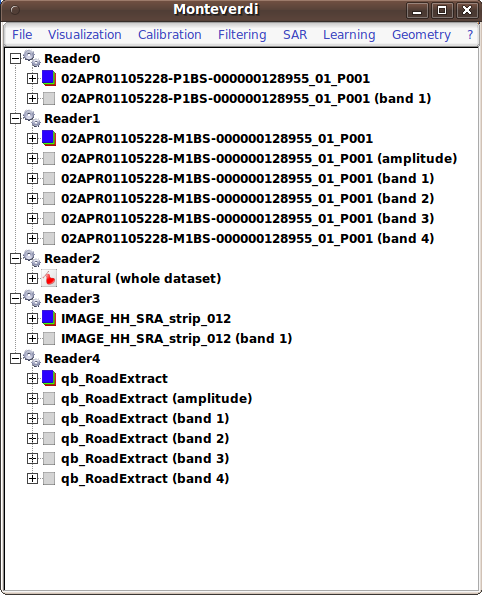
\includegraphics[width=0.44\textwidth]{monteverdi_mainwindow.eps}
   \itkcaption[Monteverdi main window]{Monteverdi main window.}
   \label{fig:mainwindow}
\end{figure}

This is Monteverdi's main window (figure \ref{mainwindow} )where the menus are available and where you can see the different 
modules which have been 
set up for the processing. Input data are obtained by readers. When you choose to use a new module, you select its input data,
 and therefore, you build a processing pipeline sequentially. 
Figure \ref{inputswindow} shows the generic window which allows to specify output(s) of Monteverdi's modules. 
 
\begin{figure}
   \center
   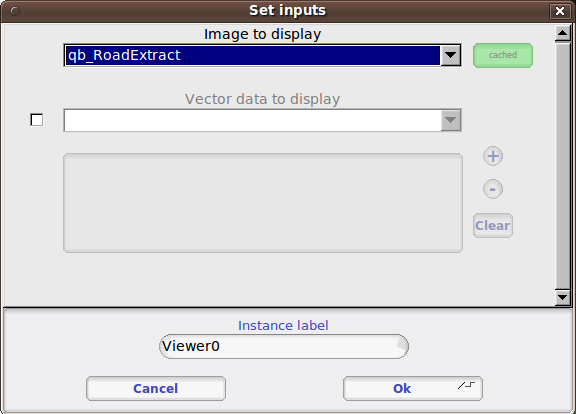
\includegraphics[width=0.44\textwidth]{monteverdi_inputs_window.eps}
   \itkcaption[Monteverdi main window]{Monteverdi inputs selection generic window.}
   \label{fig:inputswindow}
\end{figure}
Let's have a look at the different menus. The first one is of
 course the "File" menu. This menu allows you to open a data set, to save it and to cache it. The "data set" concept is
 interesting, since you don't need to define by hand if you are looking for an image or a vector file. Of course, 
you don't need to do anything special for any particular file format. So opening a data set will create a "reader" 
which will appear in the main window. At any time, you can use the "save data set" option in order to store to a 
file the result of any processing module.




\section{Open an image with Monteverdi}
The application allows to interactively select raster/vector dataset by browsing your PC. Monteverdi takes
advantage of the automatic detection of images' extensions to indicate the dataset type (optical, SAR or vector data).   

The input dataset is added to the "Data and Process" tree whcich describes the dataset content and each node corresponds to a layer.

\section{Visualize an image with Monteverdi}
This module allows to visualize raster or vector data. It allows to create RGB composition from the imput rasters. It is also possible to add 
vector dataset which are automatically reproject in the same projection of the input image or Digital Elevation informations. 

The viewer offers three types of data visualisation: 

\begin{itemize}
\item The scroll Window : to navigate quickly inside the entire scene
\item The Full resolution window: the view of the region of interest selected in the scroll window 
\item The Zoom window
\item The Pixel description: give access to dynamic informations on the current pixel pointed. Informations display are:
  \begin{itemize}
  \item The current index
  \item The pixel value 
  \item The computed value (the dynamic of hte input image is modify to get a proper visualisation
  \item The coordinates of the current pixel (long/lat)
  \item In case where there is a Internet connection available, Monteverdi displays the estimate location of the current pixel (country + city)  
  \end{itemize} 
\end{itemize}

\begin{figure}
   \center
   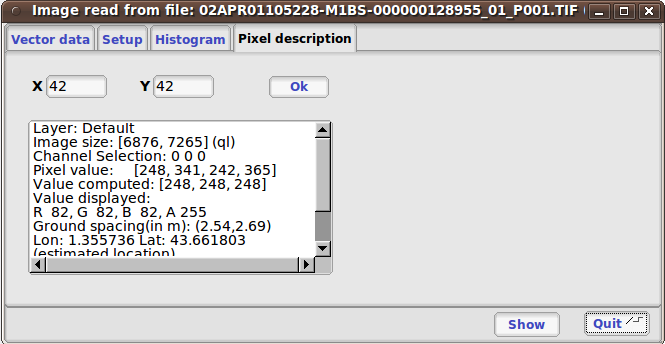
\includegraphics[width=0.44\textwidth]{monteverdi_viewer_pixel_description.eps}
   \itkcaption[Monteverdi main window]{Monteverdi pixel description box.}
   \label{fig:viewerpixeldescription}
\end{figure}

The Visualization offers others great functionnalities which are available in the detached window.
Figure \ref{viewervectordata} emphase the possibility It is possible to superpose vector dataset
to the raster image (see Figure \ref{viewervectordata}).

\begin{figure}
   \center
   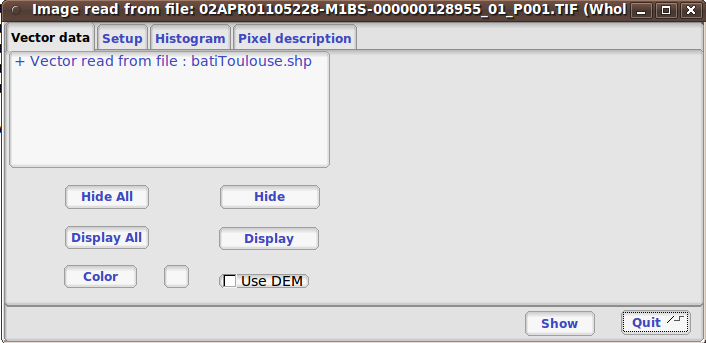
\includegraphics[width=0.44\textwidth]{monteverdi_viewer_vector_data.eps}
   \itkcaption[Vector Data visualization]{Monteverdi pixel description box.}
   \label{fig:viewervectordata}
\end{figure}

The "Setup Tab" allow to modify the RGB composition or use the grayscale mode to display only one layer. 

\begin{figure}
   \center
   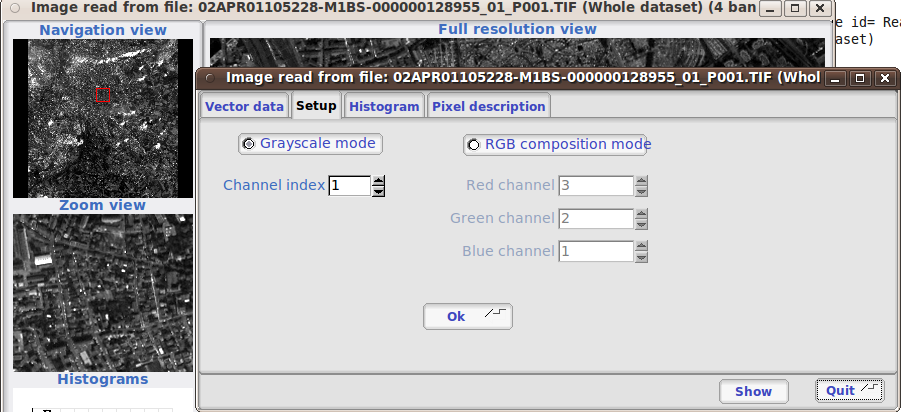
\includegraphics[width=0.44\textwidth]{monteverdi_viewer_rgb_composition.eps}
   \itkcaption[Manage RGB composition]{Manage RGB composition.}
   \label{fig:rgbcomposition}
\end{figure}

The "Histogram Tab" get access to the dynamic of the displayed layers. The basic idea is to Convert the output of the 
pixel representation to a RGB pixel on unsigned char to be displayed on screen. 
Values are contrained to 0-255 with a transfer function and a clamping operation.
By default, the dynamic of each layer is modified by
clamping the histogram at $min + 2\%$ and $max - 2\%$. 

\begin{figure}
   \center
   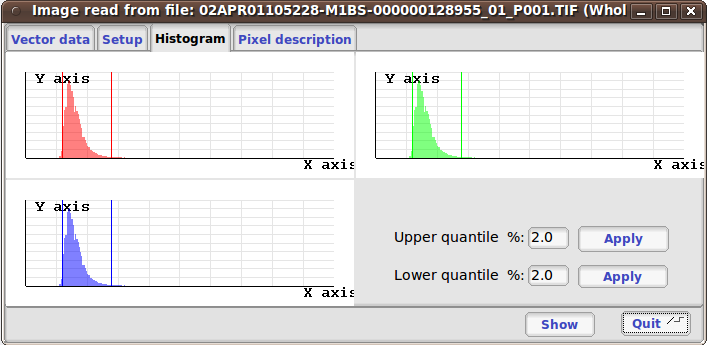
\includegraphics[width=0.44\textwidth]{monteverdi_viewer_histogram.eps}
   \itkcaption[Manage the dynamic of each layer]{Manage the dynamic.}
   \label{fig:histogram}
\end{figure}

There is also possible to select pixel coordinates and get access to all the informations abvailable in the Pixel description 
Box.

\begin{figure}
   \center
   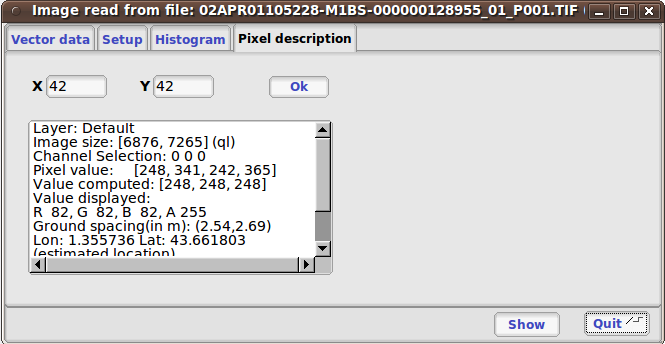
\includegraphics[width=0.44\textwidth]{monteverdi_viewer_pixel_description.eps}
   \itkcaption[Pixel description via index selection]{Index description via index selection.}
   \label{fig:pixeldescriptioninformations}
\end{figure}

\section{Cache dataset}
The "cache data set" (Figure \ref{cachingmodule}) is a very interesting thing. As you know, OTB implements processing on demand, so when you build a 
processing pipeline, no processing takes place unless you ask for it explicitly. That means that you can plug together
 the opening of a data set, an orthorectification and a spleckle filter, for example, but nothing will really be computed 
until you trigger the pipeline execution. This is very convenient, since you can quickly build a processing pipeline and 
let it execute afterwards while you have a coffee. In Monteverdi, you execute the processing by saving the result of the 
last module of a pipeline. However, sometimes, you may want to execute a part of the pipeline without wanting to give a 
name to the obtained result. You can do this by caching a data set. That is, the result will be stored in a temporary 
file which will be created in the "Caching" directory created by the application. Another situation in which you may need 
to cache a data set is when you need the input of a module to exist when you set its parameters. This is nor a real requirement, 
since Monteverdi will generate the needed data by streaming it, but this can be inefficient. This for instance about visualization
 of the result of a complex processing. Using streaming for brwsing through the result image means processing the visible part 
every time you move inside the image. Caching the data before visualization generated the whole data set in advance allowing 
for a more swift display. All modules allow you to cache their input data sets.

\begin{figure}
   \center
   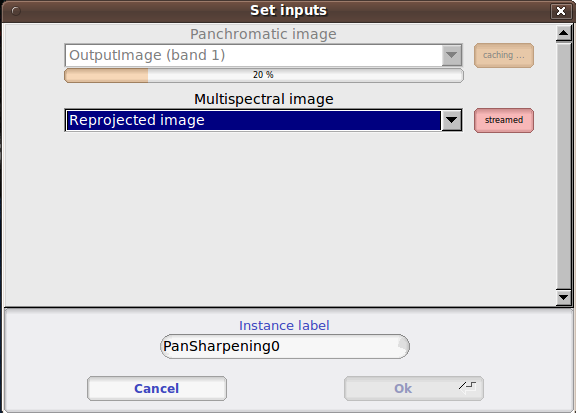
\includegraphics[width=0.44\textwidth]{monteverdi_caching_module.eps}
   \itkcaption[Cache operation on the panchromatic image in progress]{Cached and streamed dataset.}
   \label{fig:pixeldescriptioninformations}
\end{figure}

\chapter{Architecture of the application}
\section{Dynamic GUI definition}
The aim of Monteverdi is to provide a generic interface which is based on the definition of the internal processes. 
In this frame, the way that that you have to manage modules are identical during the definition of a new processes.
Selecting a module on the upper main window, open automatically the "Inputs definition Window" wich allow to select data which
are inputs of the current module. Monteverdi module can manage single or multiple inputs and these inputs can be images on your 
DD or results of previous module already registered in the "Data and Process" tree.    
\section{Dynamic I/O definition}
Management of image formats in Motneevrdi works in the manner as in the OTB library.
The principle is that the software automatically recognise the image format and.
The way that
Communication between modules follow also the same principle and the Input definition of modules request to all available
outputs of the same type in the "Data and process" tree.
Internally, all the treatments in Monteverdi are compute in Float precision by default. It is also possible to switch to Double 
precision by compiling the application from source and set the CMAKE option compile float to ON.
 

\section{Dynamic chain process}
fdsfsdfsdf

\chapter{Available modules}
\section{I/O operations}
\subsection{Extract region of interest}
It allows to extract regions of interest (ROI) from an image. There are two ways to select the region:
\begin{itemize}
\item By indicating the X and Y coordinatres of the upper-left coordinates and the X-Y size of the regions.
\item By interactivelly selecting the region of interest in the input image.
\end{itemize}

\subsection{Concatenate image bands}
With Monteverdi, you could generate a large scale of value added informations from lots of inputs data. One of the basic
functionnality is to be able to superpose result's layers into the same dataset.  
Concatenating images into one single multi-band image (they need to have the same size), and to be able to create RGB composition 
with the inputs layer.

\begin{figure}
   \center
   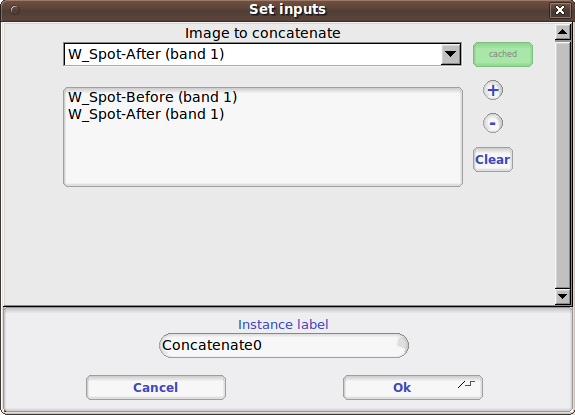
\includegraphics[width=0.44\textwidth]{monteverdi_concatenate_before_after.eps}
   \itkcaption[Concatenation of multitemporal data]{Concatenation module.}
   \label{fig:concatenate}
\end{figure}
 
\section{Geometric process}
In the frame of remote sensing process, the first operation is often to be able to superpose and maipulate imageries which 
come from different sources.
This section gives access to a large set of geometric operations.
It performs re-projection and orthorectification operations on Optical or SAR imageries using the available sensor models 
(image informations available in the meta-data are automatically read by the application).  
\subsection{Orthorectification}
The application is derived from the otbOrthorectificationApplication and allow to produce orthorectified imagery from level 1 
product.
The application is able to parse metadata informations and set default parameters. The application contains 4 tabs:

\begin{itemize}
\item Coordinates: Define the center or upper-left pixel coordinates of the orthorectified image (the Long/Lat coordinates are 
calculated through meta-data informations. It is also possible to specify the map projection of the output.
\item Output image: The module allow to only orthorectified a Region Of interest inside the input dataset. This tab allow the X and Y size 
around the center pixel coordinate or from the upper left index. The orthorectified imagery can also be resample at any resolution in the
line or column directions by setting the "Spacing X" and the "Spacing Y" and choosing the method of interpolation.
\item DEM: Indicate path to a directory containing SRTM elevation file. The application is able to detect inside the direcory which 
DEM files are relevant in the process.
\item Image extent: Compare the initial image extension with the preview the orthorectified result. This preview is automatically 
updated if the user change the "Size X" or "Size Y" values in the "Output Image" tab.   
\end{itemize}

\begin{figure}
   \center
   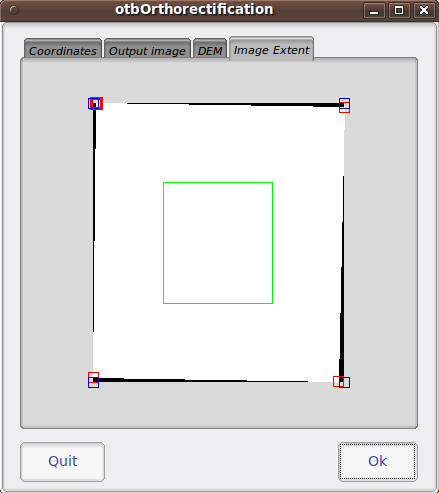
\includegraphics[width=0.44\textwidth]{monteverdi_ortho_extent.eps}
   \itkcaption[Preview of the orthorectified imagery]{Orthorectification module.}
   \label{fig:concatenate}
\end{figure}

\subsection{Re-projection module}
Allow raster reprojection of raster images.
\subsection{Registering 2 images by taking homologous point}
This module allows to register two images by taking separately homologous points in the reference image and in the image 
that you need to register. The principle is to estimate a transformation with the list of points.
The output of the module the input image that you need to register where the calculate transformation was applied. 

\begin{figure}
   \center
   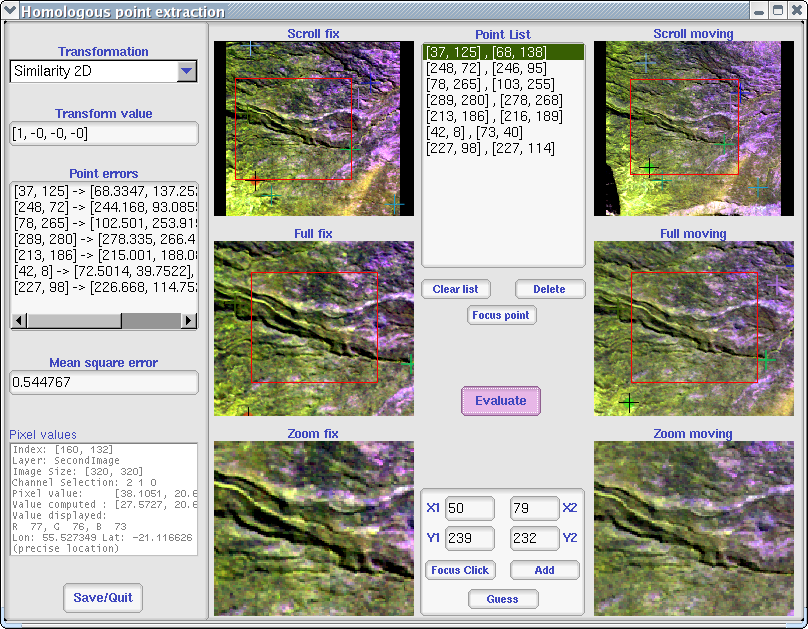
\includegraphics[width=0.44\textwidth]{monteverdi_homologous_point.eps}
   \itkcaption[Estimate transformation between 2 images]{Homologous point module.}
   \label{fig:concatenate}
\end{figure}


\subsection{Estimating sensor model based on ground control points}
This module allows to take ground copntrol points on a raster image where you 
This GCPs list is making correspondence between pixel coordinate in the input image and physical coordinates. The list
allows to derive a general function which to translate any pixel coordinates in physical positions. This function is 
based on a RPC transformation (Rational Polynomial Coefficients). As a consequence, the module enriches the output image 
with metadata informations defining a RPC sensor model associated with the input raster. 
There is several ways to generate the GCPs:

\begin{itemize}
\item With a Internet connection: Dynamically generate the correspondence on the input image and Open Street Map layers
\item Without an  Internet connection
\end{itemize}

It is also possible to import/export the GCP list from/to an XML file.

This output image could be without getting any geometric informations. Moreover, if the input image have already GCPs
in its metadata, the module allows to add or remove points from the existing list which is automatically loaded.       

\section{Calibration}
The basic idea is to be able to  
\subsection{Optical calibration}
In the case of the Optical calibration, the basic idea is to be able to retrieve reflectance of the observed physical object.
The input image contains only numerical which 
The process can be split in 3 main operations:
\begin{itemize}
\item Derived luminance from the numerical count in the input image. 
\item Convert the Luminance to Reflectance to produce the TOA(Top Of Atmosphere) image.
\item Inverse a radiative transfer code which simulate the reflection of solar radiation by a coupled atmosphere-surface system. This step produce 
the TOC (Top of Canopy) imagery which is the final result of the Optical calibration module. 
\end{itemize}
    
The module produce also a calculeted product which the TOC - TOA image.

\subsection{SAR calibration}

The calibration and validation of the measurement systems are important to maintain the
reliability and reproducibility of the SAR measurements but the establishment of correspondence between quantities measured 
by SAR and physical measure requires scientific background. The SAR calibration module allow to estimate quantitative accuracy
from Terra SAR X.
Describe the outputs!!!

\section{Filtering Operations}
\subsection{Band Math}
The Band Math module allow to perform simple mathematical operations (addition, substraction, multiplication) on 2 images. 
An operational example, on how this simple module can produce reliable information.
In rapid mapping context, it allows to compare easily . Figure XX shows the result of the substraction of water indices . The diiference was produce by the band math module
and allow to get a reliable estimation of the flood events.
\subsection{Feature extraction}
\subsection{Mean-shift segmentation}
\section{Learning}
\subsection{Supervised classification}
\subsection{Non-supervised classification}
The supervised classification  module is based on the Kmeans algorithm (link to the doc).
The GUI allows to modify parameters of the algorithm and produce
\section{Specific SAR functionnalities}
This section give access to specific treatments related to the 


\part{Developper's guide}\label{part:developperguide}
\chapter{Module architecture}
\chapter{Starter toolkit}

% \part{Appendix}\label{part:appendix}
% % \chapter{Frequently Asked Questions}
% % \label{sec:FrequentlyAskedQuestions}
% % \section{Introduction}
\subsection{What is OTB?}
OTB, the ORFEO Toolbox is a library of image processing algorithms developed by CNES in the
frame of the ORFEO Accompaniment Program.
OTB is based on the medical image processing library ITK, \url{http://www.itk.org}, and offers
particular functionalities for remote sensing image processing in
general and for high spatial resolution images in particular.

OTB provides:
\begin{itemize}
\item image access: optimized read/write access for most of remote sensing
image formats, meta-data access, simple visualization;
\item sensor geometry: sensor models, cartographic projections;
\item radiometry: atmospheric corrections, vegetation indices;
\item filtering: blurring, denoising, enhancement;
\item fusion: image pansharpening;
\item feature extraction: interest points, alignments, lines;
\item image segmentation: region growing, watershed, level sets;
\item classification: K-means, SVM, Markov random fields;
\item change detection.
\item object based image analysis.
\item geospatial analysis.
\end{itemize}

Many of these functionalities are provided by ITK and have been tested
and documented for the use with remote sensing data.

You can get more information on OTB on the web at \url{http://www.orfeo-toolbox.org}.

\subsection{What is ORFEO?}
ORFEO stands for Optical and Radar Federated Earth Observation.  In
2001 a cooperation program was set between France and Italy to develop
ORFEO, an Earth observation dual system with metric resolution: Italy
is in charge of COSMO-Skymed the radar component development, and
France of PLEIADES the optic component.

The PLEIADES optic component is composed of two "small satellites"
(mass of one ton) offering a spatial resolution at nadir of 0.7 m and
a field of view of 20 km. Their great agility enables a daily access
all over the world, essentially for defense and civil security
applications, and a coverage capacity necessary for the cartography
kind of applications at scales better than those accessible to SPOT
family satellites. Moreover, PLEIADES have stereoscopic
acquisition capacity to meet the fine cartography needs, notably in
urban regions, and to bring more information when used with aerial
photography.

The ORFEO "targeted" acquisition capacities made it a system
particularly adapted to defense or civil security missions, as well as
critical geophysical phenomena survey such as volcanic eruptions,
which require a priority use of the system resources.

With respect to the constraints of the Franco-Italian agreement,
cooperation have been set up for the PLEIADES optical component with
Sweden, Belgium, Spain and Austria.

\subsubsection{Where can I get more information about ORFEO?}
At the PLEIADES HR web site: \url{http://smsc.cnes.fr/PLEIADES/}.

\subsection{What is the ORFEO Accompaniment Program?}
Beside the Pleiades (PHR) and Cosmo-Skymed (CSK) systems developments forming ORFEO, the dual and bilateral system (France - Italy) for Earth Observation, the ORFEO Accompaniment Program was set up, to prepare, accompany and promote the use and the exploitation of the images derived from these sensors.

The creation of a preparatory program is needed because of :
\begin{itemize}
  \item the new capabilities and performances of the ORFEO systems (optical and radar high resolution, access capability, data quality, possibility to acquire simultaneously in optic and radar),
  \item the implied need of new methodological developments : new processing methods, or adaptation of existing methods,
  \item the need to realize those new developments in very close cooperation with the final users, the integration of new products in their systems.
\end{itemize}


This program was initiated by CNES mid-2003 and will last until mid 2013.
It consists in two parts, between which it is necessary to keep a strong interaction:
\begin{itemize}
\item A Methodological part,
\item A Thematic part.
\end{itemize}

This Accompaniment Program uses simulated data (acquired during airborne campaigns) and satellite images quite similar to Pleiades (as QuickBird and Ikonos), used in a communal way on a set of special sites. The validation of specified products and services will be realized with Pleiades data

Apart from the initial cooperation with Italy, the ORFEO Accompaniment
Program enlarged to Belgium, with integration of Belgian experts in
the different WG as well as a participation to the methodological
part.

\subsubsection{Where can I get more information about the ORFEO
  Accompaniment Program?}
Go to the following web site:
\url{http://smsc.cnes.fr/PLEIADES/A_prog_accomp.htm}.

\subsection{Who is responsible for the OTB development?}
The French Centre National d'\'Etudes Spatiales, CNES, initiated the ORFEO
Toolbox and is responsible for the specification of the library. CNES
funds the industrial development contracts and research contracts
needed for the evolution of OTB.

\section{License}
\subsection{Which is the OTB license?}
OTB is distributed under a CeCILL free software license:\\
\url{http://www.cecill.info/licences/Licence_CeCILL_V2-en.html} which 
is recognized by the Free Software Foundation. It can be considered 
similar to the GNU GPL license. 

\subsection{If I write an application using OTB am I forced to distribute that application?}
No. The license gives you the option to distribute your application if
you want to. You do not have to exercise this option in the license.

\subsection{If I write an application using OTB am I forced to contribute the code into the official repositories?}
No. The CeCILL license impose only to distribute the source of the application to your users.

\subsection{If I wanted to distribute an application using OTB what license would I need to use?}
The CeCILL license or the GNU GPL license.

\subsection{I am a commercial user. Is there any restriction on the
  use of OTB?}
OTB can be used internally ("in-house") without restriction, but only
redistributed in other software that is under the CeCILL license. 
Moreover you need to distribute the source of your application to your
users and only them.

\section{Getting OTB}

\subsection{Who can download the OTB?}
Anybody can download the OTB at no cost.

\subsection{Where can I download the OTB?}
Go to \url{http://www.orfeo-toolbox.org}
 and follow the "download OTB" link. You will have access to the OTB
source code, to the Software User's Guide and to the Cookbook of the last release. 
Binary packages are also provided for the current version.
OTB and Monteverdi are also integrated in OSGeo-Live since version 4.5.
You can find more information about the project at \url{http://live.osgeo.org/}. 
Moreover you can found the last release of Monteverdi and OTB applications through 
the OSGeo4W installer. 

\subsection{How to get the latest bleeding-edge version?}\label{sec:FAQMercurial}
You can get the current development version, as our repository is public, using Mercurial (available at \url{http://www.selenic.com/mercurial}). Be aware that, even if the golden rule is {\em what is committed will compile}, this is not always the case. Changes are usually more than ten per day.

The first time, you can get the source code using:
\begin{verbatim}
      hg clone http://hg.orfeo-toolbox.org/OTB
\end{verbatim}

Then you can build OTB as usual using this directory as the source (refer to build instructions).

Later if you want to update your source, from the OTB source directory, just do:
\begin{verbatim}
      hg pull -u
\end{verbatim}

A simple \texttt{make} in your OTB binary directory will be enough to update the library (recompiling only the necessary stuff).


\section{Special issues about compiling OTB from source}
\label{sec:FAQInstall}

All information about OTB compilation can be found into the related section.
We present here only the special issues which can be encountered.

\subsubsection{Debian Linux / Ubuntu}

On some Debian and Ubuntu versions, the system GDAL library and its tiff internal symbol might conflict with the system Tiff library (bugs.debian.org/558733). This is most likely the case if you get odd segmentation fault whenever trying to open a tiff image. This symbol clash happens when using OTB. A workaround to the issue has been provided in GDAL sources, but is available in the 1.9.0 release.

The recommended procedure is to get this recent source and build GDAL from sources, with the following configure command:
  \begin{verbatim}
      ./configure --prefix=INSTALL_DIR --with-libtiff=internal
                  --with-geotiff=internal
                  --with-rename-internal-libtiff-symbols=yes
                  --with-rename-internal-libgeotiff-symbol
  \end{verbatim}

\subsubsection{Errors when compiling internal libkml}
The internal version of libkml cannot be compiled when using an external build of ITK.
See \url{http://bugs.orfeo-toolbox.org/view.php?id=879} for more details.

To workaround the problem, either use an external build of libkml (it is provided on most systems), or use an internal build of ITK by setting to OFF the CMake variable OTB\_USE\_EXTERNAL\_ITK.

\subsubsection{OTB compilation and Windows platform}

To build OTB on Windows, we highly recommend using OSGeo4W which provides all the necessary dependencies.

Currently it is not possible to build OTB in Debug when using the dependencies provided by OSGeo4W.
If you want to build OTB in Debug for Windows, you will need to build and install manually each dependency needed by OTB.
You should use the same compiler for all the dependencies, as much as possible.

Therefore, we highly recommend you to use OSGeo4W shell environment to build OTB.
You can use the 32 or 64 bit installer, since OSGeo4W provides all the necessary dependencies in the two cases.
Please follow carefully the procedure provided in the Software Guide.

Typically, when using the dependencies provided by OSGeo4W, compile OTB in Release or RelWithDebInfo mode.
 
\section{Using OTB}

\subsection{Where to start ?}

OTB presents a large set of features and it is not always easy to start using it.
After the installation, you can proceed to the tutorials (in the Software Guide).
This should give you a quick overview of the possibilities of OTB and will teach
you how to build your own programs. You can also found some information in the OTB Cookbook in which we provide some recipes about remote sensing with OTB. 


\subsection{What is the image size limitation of OTB ?}

The maximum physical space a user can allocate depends on her platform. Therefore, image allocation in OTB is restricted by image dimension, size, pixel type and number of bands.

Fortunately, thanks to the streaming mechanism implemented within OTB's pipeline (actually ITK's), this limitation can be bypassed. The use of the \doxygen{otb}{ImageFileWriter} at the end of the pipeline, will seamlessly break the large, problematic data into small pieces whose allocation is possible. These pieces are processed one after the other, so that there is not allocation problem anymore. We are often working with images of $25000 \times 25000$ pixels.

For the streaming to work, all the filters in the pipeline must be streaming
capable (this is the case for most of the filters in OTB). The output image
format also need to be streamable (not PNG or JPEG, but TIFF or ENVI formats, for instance).

The class \doxygen{otb}{ImageFileWriter} manage the steaming process following two strategies: by tile or by strip. Different size configuration for these two strategies are available into the interface. The default mode use the information about how the file is streamed on the disk and will try to minimize the memory consumption along the pipeline. More information can be found into the documentation of the class. 


\section{Getting help}
\subsection{Is there any mailing list?}
Yes. There is a discussion group at
\url{http://groups.google.com/group/otb-users/} where you can get help
on the set up and the use of OTB.

\subsection{Which is the main source of documentation?}
The main source of documentation is the OTB Software Guide which can
be downloaded at
\url{http://www.orfeo-toolbox.org/packages/OTBSoftwareGuide.pdf}. It
contains tenths of commented examples and a tutorial which should be a good starting
point for any new OTB user. The code source for these examples is
distributed with the toolbox. Another information source is the
on-line API documentation which is available at \url{http://www.orfeo-toolbox.org/doxygen}.

You can also find some information about how to use Monteverdi, Monteverdi2 and the OTB-Applications into the Cookbook at \url{http://www.orfeo-toolbox.org/CookBook/}. 

\section{Contributing to OTB}\label{sec:contributing}

\subsection{I want to contribute to OTB, where to begin?}

There is many ways to join us in the OTB adventure and the more people
contribute, the better the library is for everybody!

First, you can send an email the user mailing list (otb-users@googlegroups.com)
to let us know what functionality
you would like to introduce in OTB. If the functionality seems important for the
OTB users, we will then discuss on how to retrieve your code,
make the necessary adaptions, check with you that the results are correct and finally
include it in the next release.

Then you can also run the nightly tests so we have a wider range of platforms to detect
bugs earlier. Look at section \ref{sec:runningTheTests}.

You can also find more information about how to contribute at \url{http://orfeo-toolbox.org/otb/contribute.html}

\subsection{What are the benefits of contributing to OTB?}

Besides the satisfaction of contributing to an open source project, we will include
the references to relevant papers in the software guide. Having algorithms
published in the form of reproducible research helps science move faster and
encourages people who needs your algorithms to use them.

You will also benefit from the strengths of OTB: multi-platform, streaming and
threading, etc.

\subsection{What functionality can I contribute?}

All functionalities which are useful for remote sensing data are of interest. As
OTB is a library, it should be generic algorithms: change, detection, fusion,
object detection, segmentation, interpolation, etc.

More specific applications can be contributed using the framework
directly in the Applications directory of OTB.

\section{Running the tests}\label{sec:runningTheTests}

\subsection{What are the tests?}

OTB is an ever changing library, it is quite active and have scores of
changes per day from different people. It would be a headache to make
sure that the brand new improvement that you introduced didn't break
anything, if we didn't have automated tests. You also have to take into
account differences in OS, compilers, options, versions of external
libraries, etc. By running the tests and submitting it to the dashboard,
you will help us detect problems and fix them early.

For each class, at minimum there is a test which tries to instantiate it and another one which uses the class. The output of each test (image, text file, binary file) is controlled against a baseline to make sure that the result hasn't changed.

All OTB tests source code are available in the directory \texttt{Testing} and are also good examples on how to use the different classes.

\subsection{How to run the tests?}

There is more than 2500 tests for OTB and it takes from 20 minutes to 3 hours to run all the test, mainly depending on your compilation options (Release mode does make a difference) and of course your hardware.

To run the tests, you first have to make sure that you set the option \texttt{BUILD\_TESTING} to \texttt{ON} before building the library. If you want to modify it, just rerun ccmake, change the option, then make.

For some of the tests, you also need the test data and the baselines (see \ref{sec:FAQTestData}).

Once OTB is built with the tests, you just have to go to the binary directory where you built OTB and run \texttt{ctest -N} to have a list of all the tests. Just using \texttt{ctest} will run all the tests. To select a subset, you can do \texttt{ctest -R Kml} to run all tests related to kml files or \texttt{ctest -I 1,10} to run tests from 1 to 10.

\subsection{How to get the test data?}\label{sec:FAQTestData}

Data used for the tests are also versioned using Mercurial (see \ref{sec:FAQMercurial}).

You can get the base doing:
\begin{verbatim}
      hg clone http://hg.orfeo-toolbox.org/OTB-Data
\end{verbatim}

This is about 1~GB of data, so it will take a while, but you have to do it only once, as after, a simple
\begin{verbatim}
      hg pull -u
\end{verbatim}
will update you to the latest version of the repository.

You can also easily synchronize the directory you retrieve between different computers on your network, so you don't have to get it several times from the main server. Check out Mercurial capabilities.

\subsection{How to submit the results?}

Once you know how to run the tests, you can also help us to detect the bugs or configuration problems specific to your configuration. As mentioned before, the possible combinations between OS, compiler, options, external libraries version is too big to be tested completely, but the more the better.

You just have to launch ctest with the \texttt{-D Experimental} switch. Hence:
\begin{verbatim}
      ctest -D Experimental -A CMakeCache.txt
\end{verbatim}

And you will be able to see the result at

\url{http://dash.orfeo-toolbox.org/Dashboard/index.php?project=OTB}.

If you are interested in setting up a nightly test (automatically launched every night), please contact us and we will give you the details.

\section{OTB's Roadmap}

\subsection{Which will be the next version of OTB?}
OTB's version numbers have 3 digits. The first one is for major
versions, the second one is for minor versions and the last one is for
bugfixes.

The first version was 1.0.0 in July 2006. Version 1.2.0, 1.4.0 and 1.6.0 were
released in between. The 2.0.0 major version  was released in December 2007.
The 2.2.0, 2.4.0 and 2.6.0 ({\em Halloween}) in June, July and November 2008 respectively. The
2.8.0 ({\em Gong Xi Fa Cai}) came out in January 2009, the 3.0.0 ({\em Manh\~{a} de Carnaval}) in May 2009, the 3.2.0 ({\em 62$^\circ$38${'}$35${''}$S 60$^\circ$14${'}$31${''}$W}) in January 2010, the 3.4.0 ({\em Perl A Rebours}) in July 2010, the 3.6.0 ({\em California Dreamin'}) in October 2010, the 3.8.0 ({\em Pack Ice}) in December 2010, the 3.10.0 ({\em Feli\c{c} aniversari}) in June 2011, the 3.12.0 ({\em $\Pi \lambda \epsilon l \alpha \epsilon \zeta$}) in February 2012, the 3.14.0 ({\em Happy}) in July 2012, the 3.14.1 in October 2012, the 3.16 () in February 2013 , the 3.18 ({\em Seven years of Coding}) in July 2013, the 3.18.1 in July 2013 and the 3.20 in November 2013 ({\em ... (and one more for the road)}). 

The current one is 4.0.0.

\subsubsection{What is a major version?}
A major version of the library implies the addition of high-level
functionalities as for instance image registration, object recognition, etc.

\subsubsection{What is a minor version?}
A minor version is released when low-level functionalities are
available within one major functionality, as for instance a new
change detector, a new feature extractor, etc.

\subsubsection{What is a bugfix version?}
A bugfix version is released when significant bugs are identified and fixed.

\subsection{When will the next version of OTB be available?}
We plan to release two major new OTB version once a year. You can find some information into the roadmap section of the \href{http://wiki.orfeo-toolbox.org/index.php/Main_Page}{wiki} 

\subsection{What features will the OTB include and when?}
There is no detailed plan about the availability of OTB new features,
since OTB's content depends on ongoing research work and on feedback
from thematic users of the ORFEO Accompaniment Program.

Nevertheless, the main milestones for the OTB development are the
following:
\begin{itemize}
  \item{Version 1 (2006):}
    \begin{itemize}
    \item core of the system,
    \item IO,
    \item basic filtering, segmentation and classification,
    \item basic feature extraction,
    \item basic change detection.
    \end{itemize}
    \item{Version 2 (2007):}
      \begin{itemize}
      \item geometric corrections,
      \item radiometric corrections,
      \item registration.
      \end{itemize}
    \item{Version 3 (2009):}
      \begin{itemize}
      \item multi-scale and multi-resolution analysis,
      \item object detection and recognition,
      \item supervised learning.
      \end{itemize}
    \item{Version 3.X (2010-14):}
      \begin{itemize}
	\item data fusion,
	\item spatial reasoning,
        \item hyperspectral images analysis,
        \item large scale segmentation,
        \item stereo reconstruction
        \item \ldots
      \end{itemize}
    \item{Version 4.X (2014 and later):}
      \begin{itemize}
	\item support of ITK 4.X (internal or external)
        \item Clean up: migration of FLTK related code from OTB to
          Monteverdi, remove support for pqxx, gettext and LibLAS.
      \end{itemize}

\end{itemize}

You can find more information in the \href{http://hg.orfeo-toolbox.org/OTB/file/b67d0bd93e34/RELEASE_NOTES.txt}{RELEASE\_NOTES.txt}.
%% \subsection{When will feature X or Y be included in OTB?}

% 
% \chapter{Release Notes}
% \label{sec:ReleaseNotes}
% % \verbatiminput{RELEASE_NOTES.txt}


%Comment generation of wrapping documentation for release 3.2
% \chapter{Wrappings to other languages}
%Set the code style to Java for the Wrapping

% \section{OTB-Wrapping: bindings to Java and Python languages}

This is an introduction to Wrappings concepts (mangling, template instatiation ...).

\section{Java tutorials}

\subsection{Filtering pipeline}

\input{FilteringPipelineJava.tex}

\subsection{Python}

Some python tutorials

% 
% \chapter{Contributors}
\noindent

The ORFEO Toolbox is a project conducted by CNES and developed in
cooperation with CS (Communication \& Syst\`{e}mes), \url{http://www.c-s.fr}.\\

This Software Guide is based on the ITK Software Guide: the build
process for the documentation, many examples and even the \LaTeX~ ~
sources were taken from ITK. We are very grateful to the ITK
developers and contributors and especially to Luis Ib\'a\~nez.\\

The OTB specifics were implemented and documented by the OTB Development Team
with some help from several contributors. Without these people OTB will not be
where it is today. This list is presented in alphbetical order and not by
importance of contribution:

Adamo Ferro,
Aik Song Chia (CRISP),
Alexis Huck (Magellium),
Amit Kulkarni,
Angelos Tzotsos,
Antonio Valentino,
Aur\'elien Bricier (CS),
Caroline Ruffel (CS),
Charles Peyrega (CS),
Christophe Lay,
Christophe Palmann (CS),
Conrad Bielski (JRC),
Cyrille Valladeau (CS),
David Dubois,
David Youssefi  (CNES Intern, then CS),
Edouard Barthelet (Telecom Bretagne and Thales Communications),
Emmanuel Christophe (CNES, then CRISP, then Google),
Eric Bughin (CMLA),
Etienne Bougoin (CS),
Gr\'egoire Mercier (Telecom Bretagne),
Guillaume Borrut (CS),
Guillaume Pasero (CNES Intern, then CS),
Gwendoline Blanchet (CNES),
Jan Wegner,
Jean-Guilhem Cailton (Ark\'emie),
Jens Ziehn (CNES Intern),
Jonathan Guinet (CS),
Jordi Inglada (CNES),
Julien Malik (CS),
Julien Michel (CS then CNES),
Julien Osman,
Julien Radoux (UCL),
Laurentiu Nicola (CS Romania),
Luc Hermitte (CS),
Manuel Grizonnet (CNES),
Massimo Di Stefano,
Mathieu Deltorre (CS),
Miarintsoa Ramanantsimiavona,
Michael Seymour (EADS),
Mickael Savinaud (CS),
Mohammed Rashad (CNES Intern, then CS),
Otmane Lahlou (CS),
Patrick Imbo (CS),
Remi Cresson (Irstea),
Rik Bellens,
Romain Garrigues (CS),
S\'ebastien Dinot (CS),
S\'ebastien Harasse (CS),
St\'ephane Albert (CS),
Stephane May (CNES),
Thomas Feuvrier (CS),
Tishampati Dhar,
Victor Poughon (CNES),
Vincent Poulain (CNES),
Vincent Schut (Sarvision),
Yannick Reynard


Contributions from users are expected and encouraged for the coming
versions of the ORFEO ToolBox.



\backmatter

%%%%%%%%%%%%%%%%%%%%%%%%%%%%%%%%%%%%%%%%%
%
%  Insert the bibliography using BibTeX
%
%%%%%%%%%%%%%%%%%%%%%%%%%%%%%%%%%%%%%%%%%

% \bibliographystyle{plain}
\bibliographystyle{abbrv}
\bibliography{\bibtexdatabasepath/Insight}


%%%%%%%%%%%%%%%%%%%%%%%%%%%%%%%%%%%%%%%%%
%
%  Insert the Index file
%
%%%%%%%%%%%%%%%%%%%%%%%%%%%%%%%%%%%%%%%%%

\InputIfFileExists{MonteverdiGuide.ind}




%%\ifitkPrintedVersion
%%\cleardoublepage
%%% \input{MarketingMaterial.tex}
%%\fi



\end{document}



